\section{Progress}

Where are we with design/implementation?
We've added a little scene for potential pathfinding including a goal post and starting post that a "player" would set up. 

\begin{figure}[htb]
    \centering
    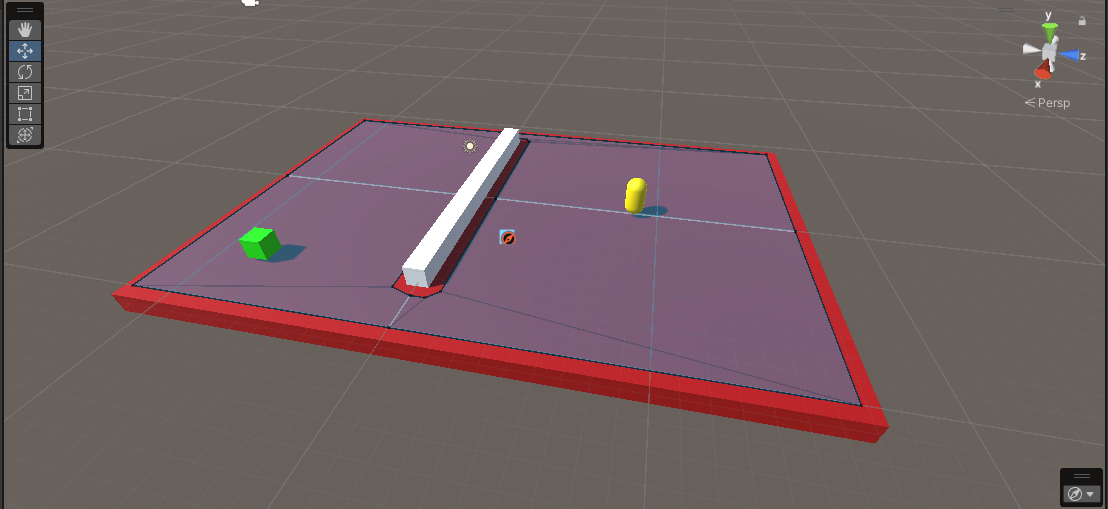
\includegraphics[width=10cm]{../Images/Update2/PathFind.png}
       \caption{A screenshot of the current pathfinding scene.}
           \label{Fig:PathfindingScene}
  \end{figure}

\begin{flushleft}
The green cube represents the post that the initial start positioned yellow capsule would make its way towards, and the white column in between is an obstacle that the NavMesh has labelled as an obstacle. In the program, the yellow capsule navigates around the column and goes towards the green goalpost. The light blue mapping on the red floor is the current NavMesh Surface baked that tells the start capsule where to go.
\end{flushleft}

\begin{figure}[!ht]
    \centering
    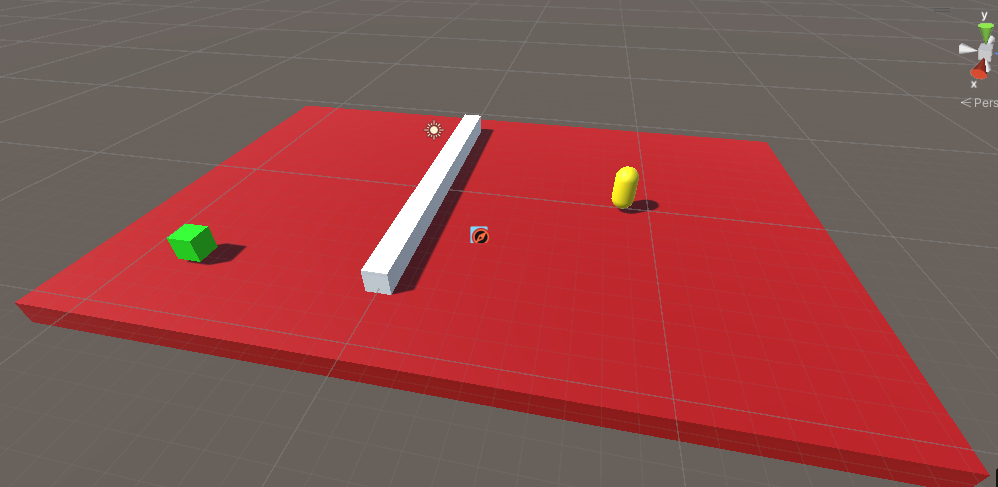
\includegraphics[width=10cm]{../Images/Update2/NoNavMesh.png}
       \caption{A screenshot of the current pathfinding scene without the NavMesh.}
           \label{Fig:NoNavMesh}
   \end{figure}

\begin{flushleft}
Currently, the two posts are set at the beginning of the project. When the game starts, the posts will be wherever they were placed before starting the game during the scene. Moving forward, we will be implementing a UI that the user can place the green goal post and place the starting yellow point and the pathfinding leads to the end. 
\end{flushleft}

We discovered a useful free Unity Asset that will make the creation of the road easier.
The asset is called EasyRoads3D Free v3 and can be found at https://assetstore.unity.com/packages/3d/characters/easyroads3d-free-v3-987

\begin{figure}[!htbp]
    \centering
    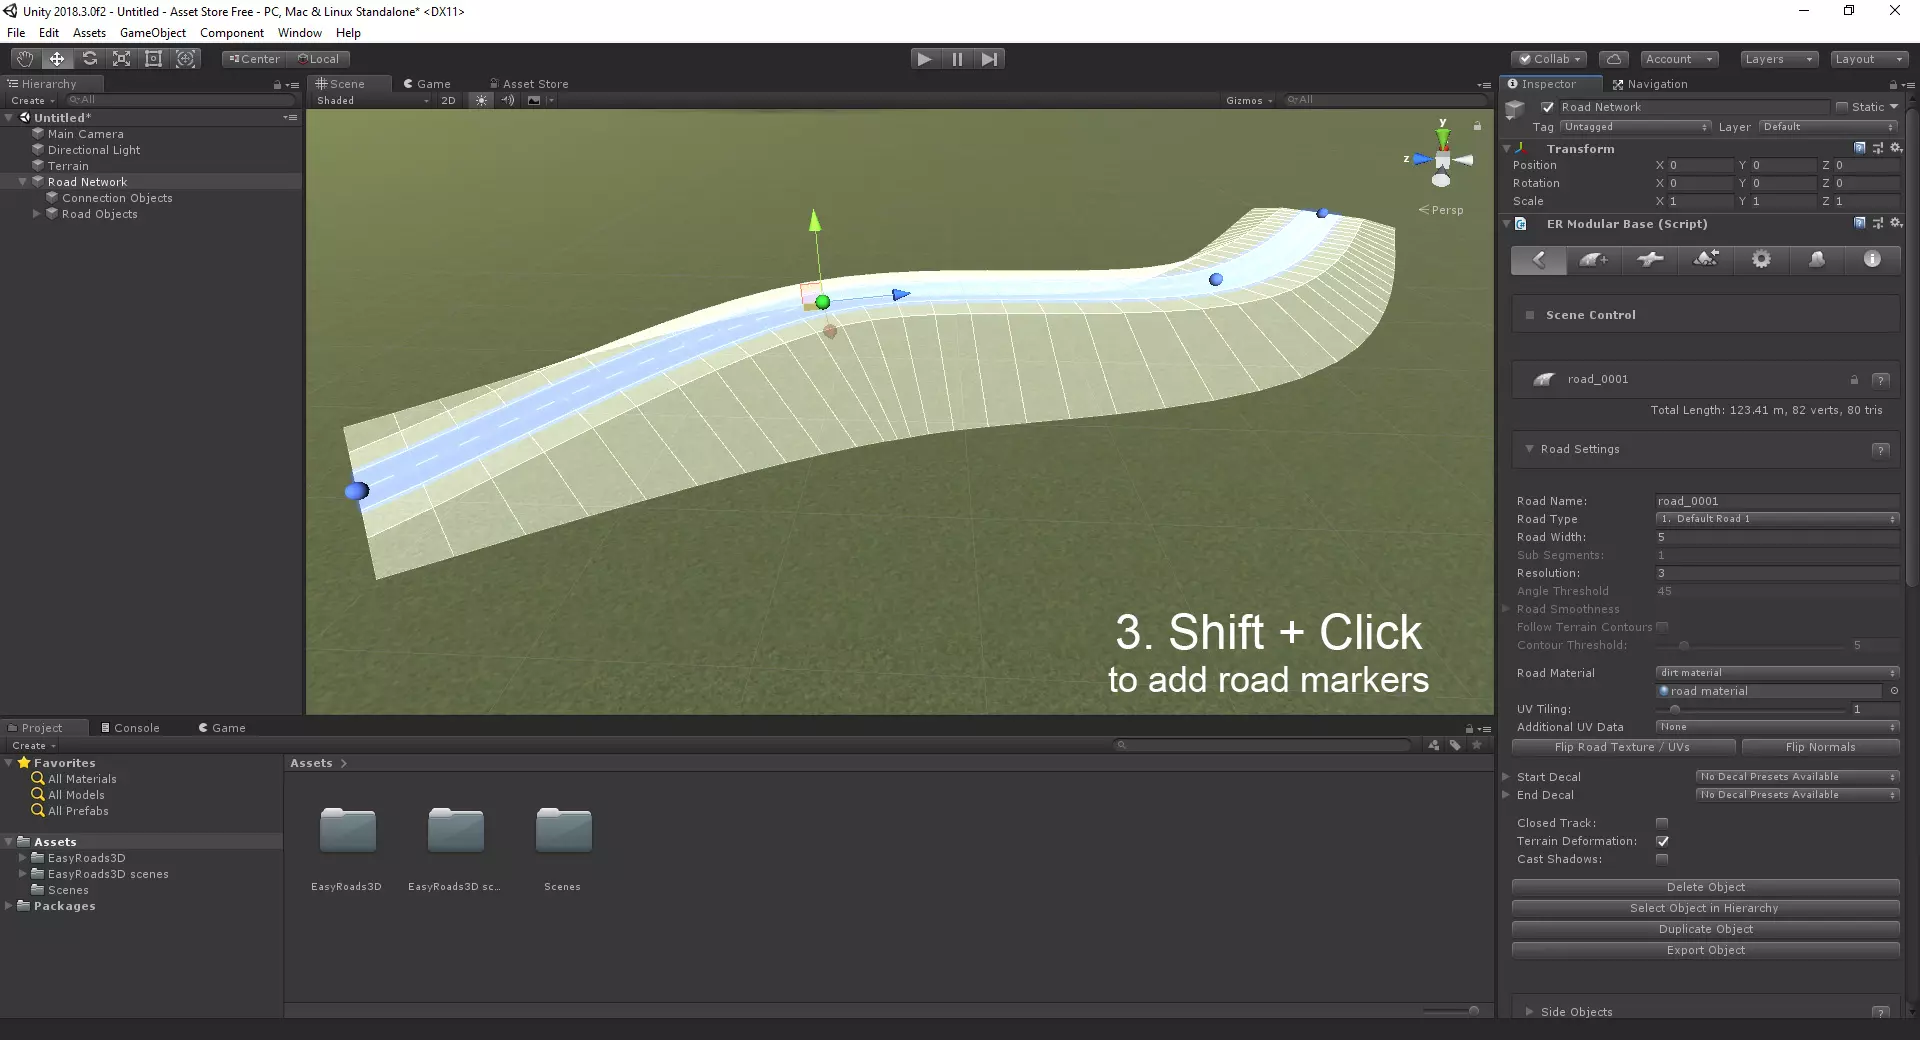
\includegraphics[width=10cm]{../Images/Update2/RoadBuild.png}
       \caption{A screenshot demoing the road creation process.}
           \label{Fig:RoadNetworkCreation}
  \end{figure}

This asset can create complex road networks based upon nodes and that means we can automate the process by placing nodes at each intersection to create a road network.

We also began to create models for our project.
Currently we have only one car modeled which is a generalized Sedan look.

\begin{figure}[!htbp]
    \centering
    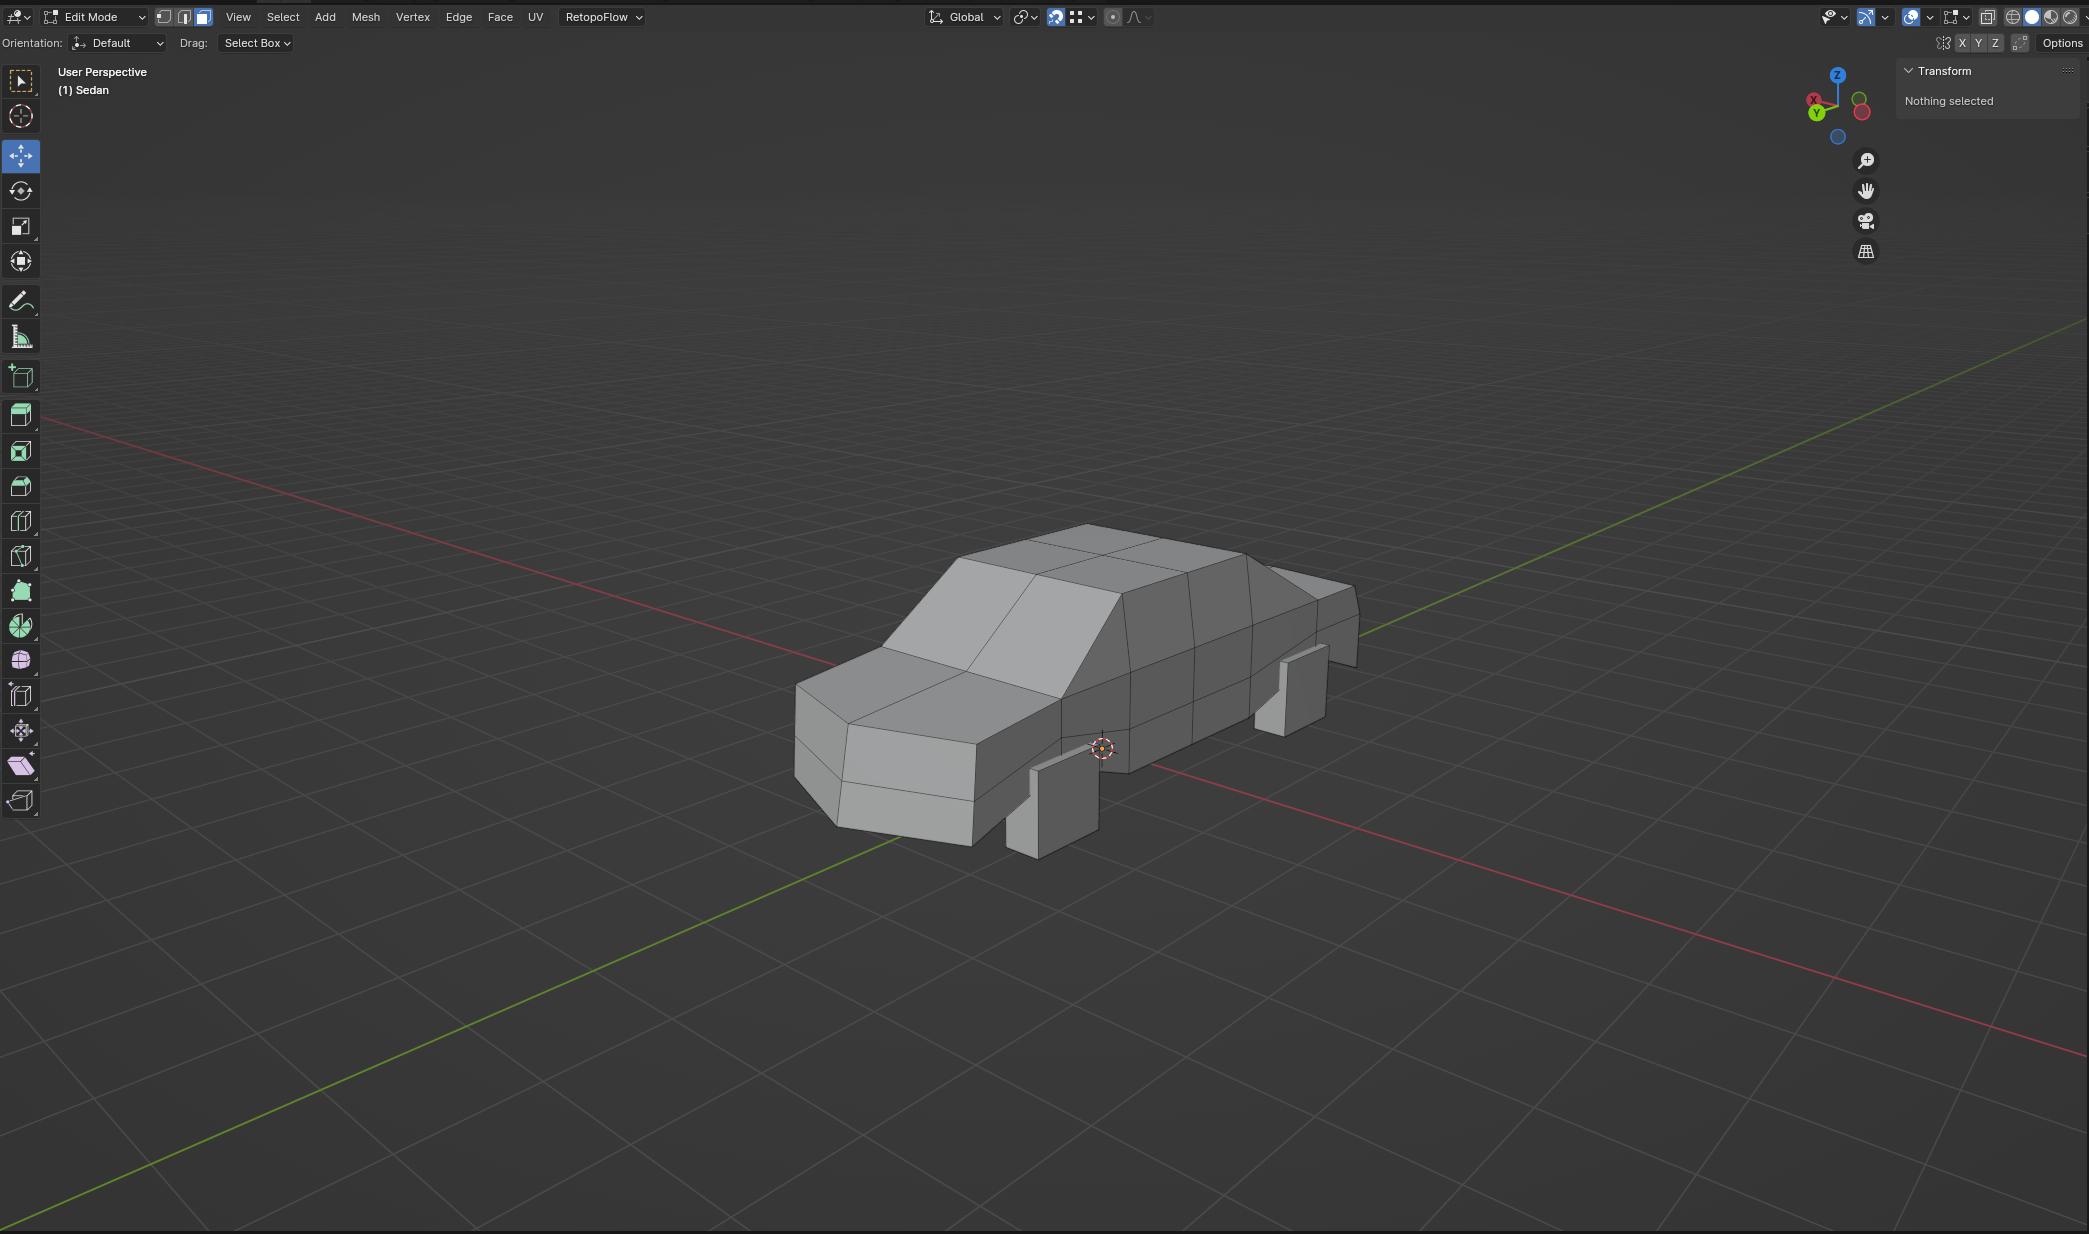
\includegraphics[width=10cm]{../Images/Update2/SedanRender.PNG}
       \caption{A screenshot of the Sedan car in Blender}
           \label{Fig:Sedan car}
  \end{figure}

Below are the packages that have been installed to allow the MLAgents git repository to be cloned.

\begin{figure}[htb]
    \centering
    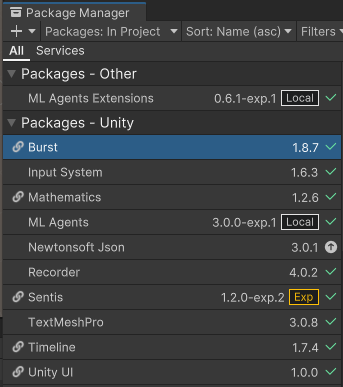
\includegraphics[width=6cm]{../Images/Update2/pkgs.png}
       \caption{Screenshot of the downloaded packages.}
           \label{Fig:Pkgs}
 \end{figure}
